\section{Théorème d'Euler}
\subsection{Énoncé du théorème}
\textit{Tout déplacement d’un corps ayant un point fixe est une rotation autour d’un
axe — fixe — passant par ce point.} 
\footnote{Source : Syllabus, page 8}\\

\subsection{Démonstration}

Afin de monter cela, on va considérer une base inertielle $\left[ \hat{\textbf{I}}\right]$, ainsi que $\left[ \hat{\textbf{x}}\right]$, une seconde base intertielle telle que $\left[ \hat{\textbf{x}}\right] = \textbf{A} \left[ \hat{\textbf{I}}\right] $. Où $A$ est une matrice de rotation\\
On va montrer qu'il existe un vecteur $\hat{\textbf{e}}$ possédant les mêmes composantes dans les deux repères. C'est à dire 
\begin{align*}
    \hat{e} &= A\hat{e}\\
    \left( A - I\right) \hat{e} &= 0
\end{align*}
C'est un problème aux valeurs propres. Il nous faut alors montrer que la matrice $A$ possède une valeur propre $\lambda = 1$ avec pour vecteur propre $\hat{\textbf{e}}$.\\

Comme $A$ est une matrice de rotation, on sait que 
\begin{itemize}
    \item $det(A) = \lambda_1 \lambda_2 \lambda_3 = 1$
    \item $A = A^T \Rightarrow A^{-1}v_i = A^T v_i =(\lambda_i)^{-1} v_i$
    \item Les valeurs propres de $A^T$ sont les mêmes que celles de $A$
\end{itemize}
On en déduit que si $\lambda'$ est une valeur propre de $A$, alors $(\lambda')^{-1}$ l'est également.
\begin{equation*}
    det(A) = \lambda' (\lambda'^{-1}) \lambda* = \boxed{\lambda* = 1}
\end{equation*}
\section{Théorême de Chasles}
\subsection{Énoncé du théorême}

Ci-dessous vous trouvez le théorême de Chasles. Cependant, il nécessite deux notions intuitives à comprendre avant de pouvoir le démontrer : \\
\begin{itemize}
    \item La rotation successive autour de deux axes $a_i$ parallèles peut s'apparenter à une rotation autour d'un axe a parallèles aux axes $a_i$.
    \item Deux rotations succesives d'angle $\alpha$ et $-\alpha$ suivants des axes parallèles est en fait une translation ! En effet, en utilisant le principe énoncé plus haut, les deux rotations peuvent s'approximer par une rotation avec le centre a rejeté à l'infini ce qui nous donne un cercle de rayon infini. Un arc de cercle très petit est approximé par un segment de droite ce qui nous donne bien une translation !
\end{itemize}
\begin{figure}[H]
    \centering
    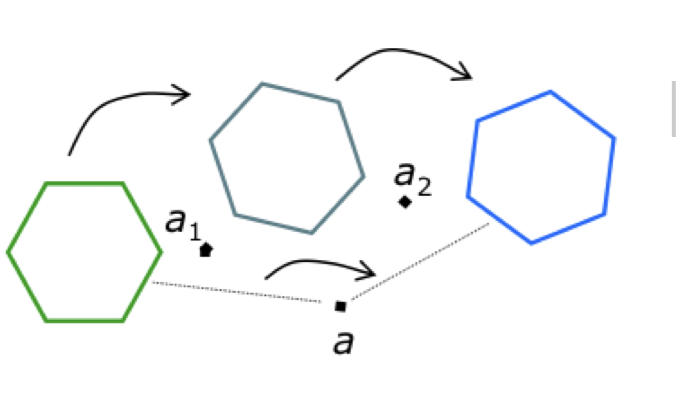
\includegraphics[width = 60 mm]{Images/imagesCinematique/Figure chasles 1.png}
    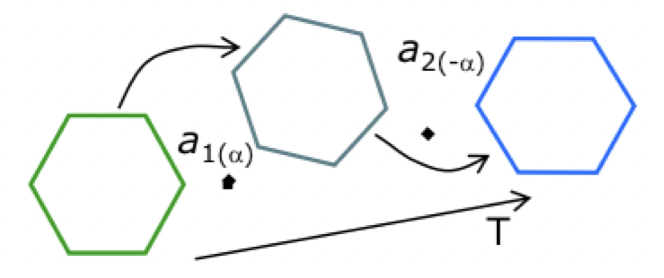
\includegraphics[width=60mm]
    {Images/imagesCinematique/Figure Chasles 2.png}
    \caption{Illustration du premier principe de Chasles}
    \label{fig:my_label}
\end{figure}
Nous pouvons donc grâce à ces deux principes énoncer le théorême de Chasles :\\

\textit{"Un déplacement fini quelconque d'un solide peut être représenté par la combinaison d'une translation et d'une rotation. Le mouvement ainsi est donc dit d'hélicoïdal."}

\section{Notions de glissement et de roulement}

\subsection{Point matériel et point géométrique}
On distingue deux types de point : 
\begin{itemize}
    \item Le point matériel, il est fixé sur un solide
    \item Le point géométrique, il n'est pas fixé et peut évoluer sur le solide au cours du temps
\end{itemize}

\section{Calcul du glissement et du roulement}

\subsection{Le glissement}

Attention, il faut faire la distinction entre glissement et frottement.
\begin{itemize}
    \item Le glissement : Vitesse relative (m/s) entre deux corps 
    \item Le frottement : Force (N) qui résulte du contact entre deux corps
\end{itemize}

\begin{figure}[H]
    \centering
    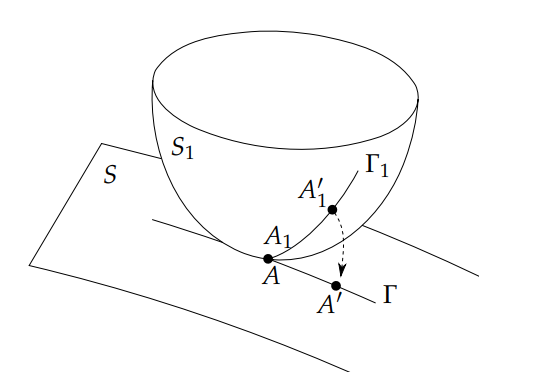
\includegraphics[width = 8cm]{Images/imagesCinematique/glissementg.png}
    \caption{bottom text}
    \label{fig:my_label}
\end{figure}
Pour comprendre ce qu'est le glissement, il faut imaginer deux coubres : 
\begin{itemize}
    \item $\Gamma$, la courbe composée de l'ensemble des points de contacts sur la surface immobile
    \item $\Gamma_1$, la courbe composée de l'ensemble des points de contacts sur le solide étudié.
\end{itemize}

On définira la vitesse de glissement $v_g$ comme la différence entre les vitesses de circulation des points de contact sur la courbe $\Gamma$ et $\Gamma_1$. En bref, c'est la vitesse relative entre la surface des deux solides en leur point de contact.

\subsection{Calculs du glissement, roulement et pivotement en pratique}


\begin{figure}[H]
    \centering
    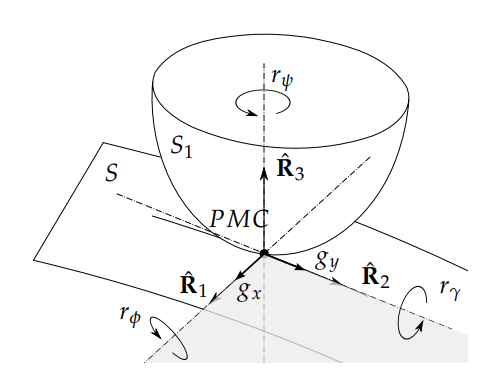
\includegraphics[width = 8cm]{Images/imagesCinematique/glissementRoulement.png}
    \label{fig:my_label}
\end{figure}

Pour calculer les glissements ($m/s$), il faut connaître la vitesse du PMC (point matériel de contact). Ensuite, il suffit de projeter cette vitesse dans le plan de contact.
\begin{align*}
    g_x &= \Vec{v}_{PMC} \cdot \hat{R}_1\\
    g_y &= \Vec{v}_{PMC} \cdot \hat{R}_2
\end{align*}

On trouve également les roulements ($rad/s$) avec les relations suivantes : 

\begin{align*}
    r_{\phi} &= \Vec{\omega}_{PMC} \cdot \hat{R}_1\\
    r_{\gamma} &= \Vec{\omega}_{PMC} \cdot \hat{R}_2\\
    r_{\psi} &= \Vec{\omega}_{PMC} \cdot \hat{R}_3
\end{align*}

\section{Mouvement général d'un solide}
\textcolor{red}{Je n'ai pas compris cette section donc je vous laisse l'écrire :-)\\
Je pense qu'il manque aussi la section sur les mouvements hélicoïdaux}

On a vu qu'un déplacement quelconque d'un solide peut être décomposé en
\begin{itemize}
    \item Une translation
    \item Une rotation parallèle à l'axe de translation.
\end{itemize}
C'est ce que l'on a appelé un déplacement hélicoïdale.\\
On va donc définir deux surfaces réglées : 
\begin{itemize}
    \item \textbf{L'axoïde fixe :} L'ensemble des droites\textit{ de l'espace} qui coïncident avec les axes hélicoïdaux. 
    \item \textbf{L'axoïde mobile :} L'ensemble des droites \textit{du solide} qui se superposent aux axes hélicoïdaux successifs. 
\end{itemize}
